\subsection{Hipótese 2}

A verificação da hipótese 2 é similar à da primeira, exceto que dessa vez segmentamos os dados em aulas que envolvem explicitamente algoritmos ou não
.
Na seção~\ref{sec:resultados} nós mostramos como essas aulas foram identificadas (coluna \foreign{algorithm} do conjunto de dados), restando agora executar a segmentação e o teste t.

\begin{figure}
	\centering
	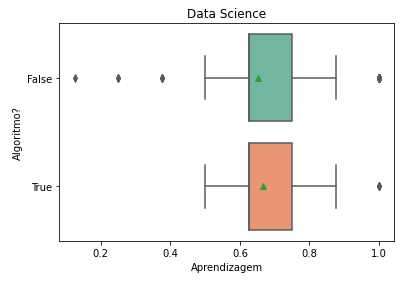
\includegraphics[width=0.45\textwidth]{ds-boxplot-by-algorithm}
	\caption{Distribuição da aprendizagem no cursos de DS para cada sub-conjunto analisado: aulas de algoritmos (\foreign{true} no eixo vertical) e as demais. Os triângulos verdes indicam a média amostral.}
	\label{fig:dist-hipotese-2}
\end{figure}

A figura~\ref{fig:dist-hipotese-2} e a tabela \ref{tab:dist-hipotese-2} apresentam a distribuição da aprendizagem das aulas de ferramentas e das demais do curso de DS.

O curso de DA não tem ênfase em algoritmos.
Por isso não propusemos fazer teste análogo nele.
De fato, podemos verificar no conjunto de dados que a quantidade de aulas com o atributo \foreign{algorithm} = \foreign{true} é zero.

Note, na tabela~\ref{tab:dist-hipotese-2}, que a média amostral das aulas de algoritmo reside no intervalo $[1,1; 1,5]$, que envolve a média amostral das demais aulas.
Além disso, os desvios-padrão são similares.
Isso evidencia que as duas amostras têm origem na mesma população.
Porém, apenas o teste t nos permitirá afirmar.

\begin{table}
	\centering
	\caption{Tamanho da amostra (\#), média (e erro padrão) e desvio-padrão das aulas de algoritmos e demais do curso de DS.}
	\label{tab:dist-hipotese-2}
	\begin{tabular}{lrrr}
		\toprule
		Algoritmo? & \# & $\bar{a}$ & $s_a$ \\
		\midrule
		Sim &  110 &  1,3(2) & 0,88 \\
		Não & 1653 & 1,25(4) & 0,88 \\
		\bottomrule
	\end{tabular}
\end{table}

\begin{table}
	\centering
	\caption{Resultado do teste t no curso de DS}
	\begin{tabular}{lcc}
	\toprule
	Curso & Valor $p$   & Estatística $t$ \\
	\midrule
	DS    & $0,41$      & $0,83$ \\ 
	\bottomrule
	\end{tabular}
\end{table}

Ao efetuarmos o teste de hipótese, obtivemos valor-$p$ de 41\%.
Ou seja, a probabilidade de observarmos a média 1,3(2) numa amostra de uma população com média 1,25(4) é de 41\%, acima do nível de significância de 5\% assumido.
Logo, podemos afirmar que as duas amostras advém da mesma população.
Consequentemente, \emph{não} há diferença de aprendizagem entre as aulas de algoritmos e as demais.